\documentclass[letterpaper, 10 pt, conference]{article} 
\usepackage[english]{babel}
\usepackage{amsmath,amssymb,amscd,amsthm} % variety of useful math macros
\usepackage[inner=1.5 cm, outer = 1.5 cm, top=1 cm, bottom = 1.5 cm]{geometry}
\usepackage{subcaption}
%For inserting graphics
\usepackage{graphicx}
\usepackage[dvipsnames]{xcolor}
\usepackage{listings}
\usepackage[utf8]{inputenc}
\usepackage{hyperref}
\usepackage{array, multirow}
\usepackage{lipsum}
\usepackage{natbib}

\bibliographystyle{abbrvnat}

\newtheorem{thm}{Theorem}
\newtheorem{prop}{Proposition}
\newtheorem{lemma}{Lemma}
\newtheorem{ex}{Exercise}

\newcommand\E{\ensuremath{\mathbb{E}}}
\newcommand\N{\ensuremath{\mathbb{N}}}
\renewcommand{\P}{\ensuremath{\mathbb{P}}}
\newcommand\Q{\ensuremath{\mathbb{Q}}}
\newcommand\R{\ensuremath{\mathbb{R}}}
\newcommand\Z{\ensuremath{\mathbb{Z}}}

\newcommand\V{\ensuremath{\mathrm{Var}}}
\newcommand\Om{\ensuremath{\Omega}}
\newcommand{\w}{\ensuremath{\omega}}

\title{Exercises
}

\hypersetup{
	colorlinks=true,
	linkcolor=blue,
	filecolor=magenta,      
	urlcolor=blue,
	citecolor=MidnightBlue
}

\author{G. Palafox}

\begin{document}
\maketitle
The following are exercises from the book of \citet{snell}.

\begin{ex}[Ex. 1, p. 247]
	A card is drawn at random from a deck consisting of cards numbered 2 through 10. A player wins 1 dollar if the number on the card is odd and loses 1 dollar if the number is even. What is the expected value of his winnings?
\end{ex}
\begin{proof}[Solution]
	We have $\Om = \lbrace 2, 3, \dots, 9, 10\rbrace$ and a random variable 
	\begin{equation}
		X(\w) = \begin{cases}
		1 & \w \text{ is odd;} \\
		-1 & \w \text{ is even.}\\
		\end{cases}
	\end{equation}
We also have $\P(\w) = 1/9$ for any card in the deck, and have exactly four odd numbers and five even numbers on said deck. Therefore, the expected value of his winnings is
\begin{equation}
	\E(X) = \sum_{\w \in \Om} X(w) \P( \w) =(-1)(1/9) +  (1/9) + \dots + (1/9) = 4(1/9) - 5(1/9) = -1/9.
\end{equation}
\end{proof}

\begin{ex}[Ex. 6, p. 247]
	A die is rolled twice. Let $X$ denote the sum of the two numbers that turn up, and $Y$ the difference of the numbers (specifically, the number on the first roll minus the number on the second). Show that $\E(XY) = \E(X) \E(Y)$. Are $X$ and $Y$ independent?
\end{ex}
\begin{proof}[Solution]
	Let $\Om = \lbrace 1, 2, \dots, 6\rbrace \times  \lbrace 1, 2, \dots, 6\rbrace$, and $X(\w_1 , \w_2) = \w_1 + \w_2, Y(\w_1, \w_2) = \w_1 - \w_2$. Define a new random variable $Z = XY$, that is, $Z(\w_1, \w_2) = (\w_1 + \w_2)(\w_1 - \w_2) = \w_{1}^{2} - \w_{2}^{2}$. Now, we have
	\begin{align}
		\E(XY) = \E(Z) &= \sum_{(\w_1, \w_2) \in \Om} \frac{1}{36} (\w_{1}^{2} - \w_{2}^{2})\\
		&= \frac{1}{36} \left( (1^2 - 1^2) + (1^2 - 2^2) + \dots + (2^2 - 1^2) + \dots + (6^2 - 1^2) + \dots (6^2 - 6^2) \right)\\
		&= \frac{1}{36} \left\lbrack \left(6(1^2) - \sum_{i = 1}^{6} i^2\right) + \left(6(2^2) - \sum_{i= 1}^{6} i^2\right) + \dots + \left(6(6^2) - \sum_{i=1}^{6} i^2\right)\right\rbrack\\
		&= \frac{1}{36} \left( 6(1^2 + \dots + 6^2) -6 \sum_{i=1}^{6} i^2\right)\\
		&= \frac{1}{36} \left(6 \sum_{i=1}^{6} i^2 - 6 \sum_{i=1}^{6} i^2\right)\\
		&= 0.
	\end{align}
 With a similar calculation, we can see that
 	\begin{align}
	\E(Y) &= \sum_{(\w_1, \w_2) \in \Om} \frac{1}{36} (\w_{1} - \w_{2})\\
	 &= \frac{1}{36} \left( (1-1) + (1-2) + \dots + (2-1) + \dots + (6-1) + \dots (6-6) \right)\\
	 &= \frac{1}{36} \left\lbrack \left(6(1) - \sum_{i = 1}^{6} i\right) + \left(6(2) - \sum_{i= 1}^{6} i\right) + \dots + \left(6(6) - \sum_{i=1}^{6} i\right)\right\rbrack\\
	 &= \frac{1}{36} \left( 6(1 + \dots + 6) -6 \sum_{i=1}^{6} i\right)\\
	 &= \frac{1}{36} \left(6 \sum_{i=1}^{6} i - 6 \sum_{i=1}^{6} i\right)\\
	 &= 0.
 \end{align}
 With this we can see that, regardless of the value of $\E(X)$ we will have 
  \begin{equation}
  	\E(X) \E(Y) = \E(X) \cdot 0 = 0 = \E(Z) = \E(XY).
  \end{equation}
  \textbf{The random variables are not independent}. To see this, consider $\P(X = 2, Y = 0)$. There is only one pair of $(\w_1, \w_2) \in \Om$ such that $\w_1 + \w_2 = 2$ and $\w_1 - \w_2 = 0$, namely $(1,1)$, so $\P(X = 2, Y = 0) = 1/36$. In fact, $\P(X = 2) = 1/36$ too. However, $\P(Y = 0) = 6/36$, for every pair $(\w_1, \w_2)$ with $\w_1 = \w_2$ satisfies, so 
  \begin{equation}
  	\P(X = 2) \P(Y = 0) = (1/36)(6/36) \neq \P(X = 2, Y = 0) = 1/36.
  \end{equation}
\end{proof}

\begin{ex}[Ex. 18, p. 249]\label{ex:keys}
Exactly one of six similar keys opens a certain door. If you try the keys, one after another, what is the expected number of keys that you will have to try before success?
\end{ex}
\begin{proof}[Solution]
Lets denote by 0 choosing a wrong key, and by 1 choosing the correct key. Then 
\begin{equation}
\Om = \lbrace 1, 01, 001, 0001, 00001, 000001 \rbrace,
\end{equation}
and $X(\w) = \textit{number of zeros in } \w$. Assuming the keys are chosen uniformly at random, and that once a key is tried we discard it (i.e., \textit{no replacement}), the probabilities of trying $k$ keys before success are as seen in Table \ref{tab:ex3}.

\begin{table}
\centering
\begin{tabular}{|c|c|}
	\hline
	$k$ & $\P(X = k)$ \\
	\hline
	$0$ & $\frac{1}{6}$ \\
	\hline
	$1$ & $\frac{5}{6} \cdot \frac{1}{5} = \frac{1}{6}$ \\
	\hline
	$2$ &  $\frac{5}{6} \cdot \frac{4}{5} \cdot \frac{1}{4} = \frac{1}{6}$ \\
	\hline
	$3$ & $\frac{5}{6} \cdot \frac{4}{5} \cdot \frac{3}{4} \cdot \frac{1}{3} = \frac{1}{6}$ \\
	\hline
	$4$ & $\frac{5}{6} \cdot \frac{4}{5} \cdot \frac{3}{4} \cdot \frac{2}{3} \cdot \frac{1}{2} = \frac{1}{6}$  \\
	\hline
	$5$ & $\frac{5}{6} \cdot \frac{4}{5} \cdot \frac{3}{4} \cdot \frac{2}{3} \cdot \frac{1}{2} \cdot 1 = \frac{1}{6}$ \\
	\hline
\end{tabular}
\caption{Probabilities for Exercise \ref{ex:keys}}
\label{tab:ex3}
\end{table}


Thus, the expected number of keys to try before success is
\begin{align}
	\E(X) &= \sum_{k = 0}^{5} (1/6) k\\
	&= \frac{1}{6} \sum_{k = 0}^{5} k\\
	&= \frac{1}{6} \cdot 15 \\
	&= 2.5
\end{align}
\end{proof}


\begin{ex}[Ex. 19, p. 249]
	A multiple choice exam is given. A problem has four possible answers, and exactly one answer is correct. The student is allowed to choose a subset of the four possible answers as his answer. If his chosen subset contains the correct answer, the student receives three points, but he loses one point for each wrong answer in his chosen subset. Show that if he just guesses a subset uniformly and randomly his expected score is zero. 
\end{ex}
\begin{proof}[Solution]
Let $A$ be the four-element-set of possible answers for the question. Then our sample space is the power set $\Om = 2^A$, and $X(\w) = \textit{points received by choosing the subset } \w$. Denote by $|\w|$ the cardinality of a subset $\w \in \Om$. Then we have 
\begin{equation}\label{expected_points_subsets}
	\E(X) = \sum_{\w \in \Om} \frac{1}{16} \left( \frac{|w|}{4} \left(3 - (|\w| - 1)\right) - \left(1-\frac{|\w|}{4}\right) |\w| \right).
\end{equation}
To explain Equation \ref{expected_points_subsets}, see that the probability of a subset $\w$ containing the right answer is $|\w| / 4$, in which case, the student would get $3-(|\w| -1)$ points, three for the right answer and minus one for each of the $|\w| - 1$ wrong answers. On the other hand, the probability of a subset not containing the answer is $1-\frac{|\w|}{4}$ and the student would lose $|\w|$ points.  Observe that 
\begin{align}
 \frac{|w|}{4} \left(3 - (|\w| - 1)\right) - \left(1-\frac{|\w|}{4}\right) |\w| &=  \frac{|w|}{4}  \left(3 - |\w| + 1\right) - \left(\w - \frac{|\w|^2}{4}\right)\\
 &= \frac{3 |\w|}{4} - \frac{|\w|^2}{4} + \frac{|\w|}{4} - |\w| + \frac{|\w|^2}{4}\\
 &= 0.
\end{align}
Therefore, the expected score for the student is 
\begin{equation}
	\E(X) = \sum_{\w \in \Om} \frac{1}{16} (0) = 0.
\end{equation}
\end{proof}

\begin{ex}[Ex. 31, p. 254]
A large number, $N$, of people are subjected to a blood test. This can be administered in two ways: (1) Each person can be tested separately, in this case $N$ tests are required, (2) the blood samples of $k$ persons can be pooled and analyzed together. If this test is \textit{negative}, this one test suffices for the $k$ people. If the test is positive, each of the $k$ persons must be tested separately, and in all, $k+1$ tests are required for the $k$ people. Assume that the probability $p$ that a test is positive is the same for all people and that these events are independent.
\begin{enumerate}
	\item Find the probability that the test for a pooled sample of $k$ people will be positive. 
	\item What is the expected value of the number $X$ of tests necessary under plan (2)? (Assume that $N$ is divisible by $k$.)
	\item For small $p$, show that the value of $k$ which will minimize the expected number of tests under the second plan is approximately $1/\sqrt{p}$.
\end{enumerate}
\end{ex}
\begin{proof}[Solution]
Since each of the $k$ persons have a probability $p$ of being positive, the probability that at least one of them is positive (and hence, the pool) is $p + p + \dots + p = kp$.

Under plan (2), we have an expected number of tests of
\begin{align}
	\E(X) &= \sum_{i = 1}^{N/k} kp(k+1) + (1-kp) \\
	&= (N/k) \lbrack kp (k+1) + (1-kp)\rbrack\\
	&= Np(k+1) + N/k - Np\\
	&= Npk + N/k.
\end{align}
To minimize this expected value with a fixed $N$ and $p$, we consider the expected value as a function of $k, f(k) = Npk + N/k$. The function has derivative $f'(k) = Np - \frac{N}{k^2}$, which is zero in $k=1/\sqrt{p}$, and second derivative $f''(k) = N/k^3$, which is positive for $k = 1/\sqrt{p}$, so $k = 1/\sqrt{p}$ minimizes the expected value. For this value to make sense, $k$ must be greater than two, so $p$ must be small.
\end{proof}

\begin{ex}[Ex. 1, p. 263]
	A number is chosen at random from the set $S = \lbrace -1, 0, 1\rbrace$. Let $X$ be the number chosen. Find the expected value, variance and standard deviation of $X$. 
\end{ex}
\begin{proof}[Solution]
	We have 
	\begin{equation}
	\E(X) = (1/3)(-1) + (1/3)(0) + (1/3)(1)= 0,
	\end{equation}
	so
	\begin{equation}
		\V(X) = \E[ (X-\mu)^2] = \E(X^2) = (1/3)(1) + (1/3)(0) + (1/3)(1) = 2/3,
	\end{equation} 
	and $D(X) = \sqrt{\V(X)} = \sqrt{2/3} $.
\end{proof}

\begin{ex}[Ex. 9, p. 264]
	A die is loaded so that the probability of a face coming up is proportional to the number on that face. The die is rolled with outcome $X$. Find $\V(X)$ and $D(X)$. 
\end{ex}
\begin{proof}[Solution]
	Since $1+2+\dots+6 = 21$,, we make $\P(X = k) = k/21$. With this, 
	\begin{align}
		\E(X) &= \sum_{k = 1}^{6} k \P(X = k)\\
		&= \sum_{k = 1}^{6} k (k/21)\\
		&= (1/21) \sum_{k = 1}^{6} k^2 \\
		&= (1/21) \frac{6 \cdot 7 \cdot 13}{6}\\
		&= (1/21) (91) \\
		&= 13/3 \\
		&\approx 4.333,
	\end{align}
	so 
	\begin{align}
		\V(X) &= \sum_{k = 1}^{6} \lbrack (k-13/3)^2 (k/21) \rbrack\\
		&= \sum_{k = 1}^{6} \lbrack (k^2 - 2k(13/3) + (13/3)^2) (k/21) \rbrack\\
		&= \sum_{k = 1}^{6} \lbrack \frac{k^3}{21} - 2 (\frac{13}{3 \cdot 21}) k^2 + (\frac{13}{3})^2 \frac{k}{21} \rbrack \\
		&= \frac{1}{21} \sum_{k = 1}^{6}  k^3 - 2 (\frac{13}{3 \cdot 21}) \sum_{k = 1}^{6} k^2 + \frac{1}{21}(\frac{13}{3})^2 \sum_{k = 1}^{6} k \\
		&= \frac{1}{21} (\frac{36 \cdot 49}{4}) - \frac{2 \cdot 13}{3 \cdot 21} (91) + \frac{1}{21} (13/3)^2 (21)\\
		&= 9 (7/3) - 2 (13/3)^2 + (13/3)^2\\
		&= 20/9\\
		&\approx 2.222,
	\end{align}
	and $D(X) = \sqrt{\V(X)} = \sqrt{20/9} = \sqrt{20}/3 \approx 1.49$.
\end{proof}

\begin{ex}[Ex. 12, p. 264]
	Let $X$ be a random variable with $\mu = \E(X)$ and $\sigma^2 = \V(X)$. Define $X^\ast = (X-\mu)/\sigma$. The random variable $X^\ast$ is called the \textit{standardized random variable} associated with $X$. Show that this standardized random variable has expected value 0 and variance 1.
\end{ex}
\begin{proof}[Solution]
	Theorem 6.2 from \citet{snell} tells us that, for random variables $X, Y$ with finite expected values, we have 
	\begin{equation}
		\E(X+Y) = \E(X) + \E(Y),
	\end{equation}
	and if $c$ is any constant, then
	\begin{equation}
		\E(cX) = c\E(X).
	\end{equation}
	Therefore, 
	\begin{align}
		\E(X^\ast) &= \E\lbrack(X-\mu)/\sigma\rbrack\\
		&= \frac{1}{\sigma} \E(X - \mu)\\
		&= \frac{1}{\sigma} (\E(X) - \E(\mu))\\
		&= \frac{1}{\sigma} (\mu - \mu)\\
		&= 0,
	\end{align}
	and, writing $\mu^\ast$ for $\E(X^\ast)$, 
	\begin{align}
		\V(X^\ast) &= \E\lbrack(X^\ast - \mu^\ast)^2\rbrack\\
		&= \E\lbrack(X^\ast)^2\rbrack\\
		&= \E\lbrack \frac{(X-\mu)^2}{\sigma^2}\rbrack\\
		&= \frac{1}{\sigma^2} \E\lbrack(X-\mu)^2\rbrack\\
		&= \frac{1}{\sigma^2} \V(X)\\
		&= \frac{1}{\sigma^2}\sigma^2 = 1.
	\end{align}
\end{proof}

\begin{ex}[Ex. 3, p. 278]
	The lifetime, measured in hours, of the ACME super light bulb is a random variable $T$ with density function $f_T (t) = \lambda^2 t e^{-\lambda t}$, where $\lambda = 0.05$. What is the expected lifetime of this light bulb? What is its variance?
\end{ex}
\begin{proof}[Solution]
	The expected lifetime will be given by
	\begin{equation}
		\E(T) = \int_{0}^{\infty} t (\lambda^2 t e ^{-\lambda t}) dt.
	\end{equation}
First, the indefinite integral is solved. This is rewritten as
	\begin{equation} \label{int_parts_1}
		\int t (\lambda^2 t e ^{-\lambda t}) \, dt = (-\lambda) \int t^2 (-\lambda e ^{-\lambda t}) \, dt,
	\end{equation}
	and integrating by parts gives
	\begin{equation} \label{int_parts_2}
		\int t^2 (-\lambda e ^{-\lambda t}) \, dt = t^2 e^{-\lambda t} - \int (2t) e^{-\lambda t} dt.
	\end{equation}
	Substituting Equation \ref{int_parts_2} in \ref{int_parts_1} we obtain:
	\begin{equation}\label{int_parts_3}
			\int t (\lambda^2 t e ^{-\lambda t}) \, dt = -\lambda t^2 e^{-\lambda t} - 2 \int t (-\lambda e^{-\lambda t}) \, dt.
	\end{equation}
	The integral in Equation \ref{int_parts_3} can be done via integration parts too, as
	\begin{equation} \label{int_parts_4}
		\int t (-\lambda e^{- \lambda t} ) \, dt = t e^{\lambda t} - \int e^{-\lambda t} \, dt
		= t e^{- \lambda t} + \frac{1}{\lambda} e^{-\lambda t}.
	\end{equation}
	Putting the result of Equation \ref{int_parts_4} in \ref{int_parts_3} gives
	\begin{align}\label{int_parts_5}
		\int t (\lambda^2 t e ^{-\lambda t}) \, dt = -\lambda t^2 e^{-\lambda t} - 2 t e^{-\lambda t} - \frac{2}{\lambda} e^{-\lambda t}.
	\end{align}
	Denoting the resulting function of Equation \ref{int_parts_5} as $F(t)$, we have 
	\begin{equation}
		\E(T) = \lim_{t \longrightarrow \infty} F(t) - F(0) = \frac{2}{\lambda}.
	\end{equation}
	Therefore, the\textbf{ expected lifetime of this light bulb} is $2/0.05 = 40$ hours. To find the variance, first $\E(T^2)$ will be obtained. This is equal to 
	\begin{equation}
		\int_{0}^{\infty} t^2(\lambda t e^{-\lambda t}) \, dt = \int_{0}^{\infty} \lambda^2 t^3 e^{-\lambda t} \, dt.
	\end{equation}
	As before, the indefinite integral is calculated first. First, it is observed that
	\begin{equation}\label{int_parts_21}
		 \int \lambda^2 t^3 e^{-\lambda t} \, dt = -\lambda \int t^3 (-\lambda e^{-\lambda t} )\, dt,
	\end{equation}
	and integrating by parts gives
	\begin{equation}\label{int_parts_22}
		\int t^3 (-\lambda e^{-\lambda t} )\, dt = t^3 e^{-\lambda t} - \int 3 t^2 e^{-\lambda t} \, dt.
	\end{equation}
	Therefore, substituting the result of Equation \ref{int_parts_22} in Equation \ref{int_parts_21}, we obtain
	\begin{equation}\label{int_parts_23}
		\int \lambda^2 t^3 e^{-\lambda t} dt = -\lambda t^3 e^{-\lambda t} + 3 \int \lambda t^2 e^{-\lambda t} \, dt.
	\end{equation}
 	From Equation \ref{int_parts_5}, we know
	\begin{equation}
		\int \lambda t^2 e^{-\lambda t} \, dt = \frac{1}{\lambda} \int \lambda^2 t^2 e^{-\lambda t} \, dt =  \frac{1}{\lambda} F(t),
	\end{equation}
	thus
	\begin{equation}
		\int \lambda^2 t^3 e^{-\lambda t} \, dt = -\lambda t^3 e^{-\lambda t} + \frac{3}{\lambda} F(t), 
	\end{equation}
	and
	\begin{equation}
		\E(T^2) = \lim_{t \longrightarrow \infty} (-\lambda t^3 e^{-\lambda t} + \frac{3}{\lambda} F(t) + \frac{3}{\lambda} \frac{2}{\lambda}) = \frac{6}{\lambda^2}.
	\end{equation} 
	Now, by Theorem 6.15 \citep{snell}, $\V(T) = \E(T^2) - \E(T)^2$, so we get $\V(T) = \frac{6}{\lambda^2} - (\frac{2}{\lambda})^2$. In this particular example, $\lambda = 0.05$, which gives a variance $\V(T) = 2400-1600=800$.
\end{proof}

\begin{ex}[Ex. 26, p. 284] \label{ex:river}
Suppose you are standing on the bank of a straight river.
\begin{enumerate}
	\item Choose, at random, a direction which will keep you on dry land, and walk 1 km in that direction. Let $P$ denote your position. What is the expected distance from $P$ to the river?
	\item Now suppose you proceed as in part (1), but when you get to $P$, you pick a random direction (from among \textit{all} directions) and walk 1 km. What is the probability that you will reach the river before the second walk is completed?
\end{enumerate}
\end{ex}
\begin{proof}[Solution]
	In part 1, the possible directions to stay on dry land are given by $\theta, 0 \leq \theta \leq \pi$. By basic trigonometry, the distance between the river and the point $P$ resulting from walking 1 km in a $\theta$-radian direction is $\sin \theta$. Since this $\theta$ is chosen uniformly at random, the expected distance is 
	\begin{equation}
		\int_{0}^{\pi} \frac{1}{\pi} \sin( \theta) \, d\theta = \frac{2}{\pi}.
	\end{equation}
	In part 2, we need to know in which directions is the river less than 1 km away. These are the directions inside the triangle in Figure \ref{fig:river}, which forms a $\pi - 2\theta$ radians angle. The probability of choosing any of these directions is $\frac{\pi-2\theta}{2\pi} = \frac{1}{2} - \frac{\theta}{\pi}$.
\end{proof}

\begin{figure}
	\centering
	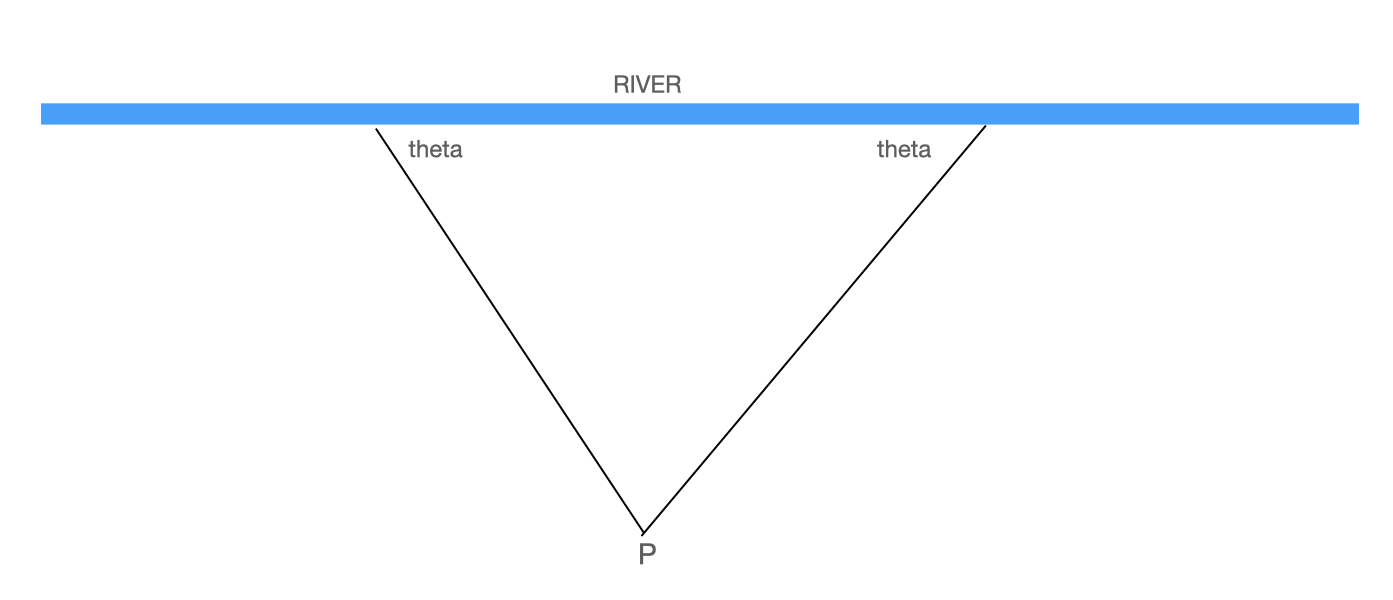
\includegraphics[width=0.6\linewidth]{river_problem}
	\caption{Figure for Exercise \ref{ex:river}}
	\label{fig:river}
\end{figure}

\begin{ex}[Ex. 27, p. 284]
A game is played as follows: A random number $X$ is chosen uniformly from $[0,1]$. Then a sequence $Y_1, Y_2, \dots$ of random numbers is chosen independently and uniformly from $[0,1]$. The game ends the first time that $Y_i > X$. You are then paid $(i-1)$ dollars. What is a fair entrance fee for this game?
\end{ex}
\begin{proof}[Solution]
First, let's establish that if $Z$ is the payout from playing the game, we will consider $E(Z)$ a fair entrance fee, since anything larger than $E(Z)$ would be disadvantageous to the player, and anything less than $E(Z)$ would be unfair to whomever is running the game. Now, to calculate the expected gain, see that for any $Y_i, \, \P(Y_i < X) = X$ and $\P(Y_i \geq X) =  1-X$. Hence, the probability of ending the game in $k$ steps would be $X^{k-1} (1-X)$, therefore
\begin{align}
	E(Z) &= \sum_{k = 1}^{\infty} (k-1) X^{k-1}(1-X)\\
	&= \sum_{k = 0}^{\infty} k X^k(1-X) \\
	&=  \sum_{k = 0}^{\infty} k X^k -  \sum_{k = 0}^{\infty} k X^{k+1}\\
	&= \frac{X}{(X-1)^2} - \frac{X^2}{(X-1)^2}\\
	&= \frac{X - X^2}{(X-1)^2}\\
	&= \frac{-X}{X-1} = \frac{X}{1-X}.
\end{align}
Since $\E(X) = 1/2$, then $E(Z) = \frac{1/2}{1-1/2} = 1$ would be a fair entry fee.
\end{proof}

%%%%%%%%%%%%%%%%%%%%%%%%%%%%%%%%%%%%%%%%%%%%%%%%%%%%%%%%%%%%%%%%%%%%%%%%%%%%%%%%

\bibliography{ref}

\end{document}
